
\begin{figure}[h]
% \vskip -0.2in
  \centering
  \begin{subfigure}[t]{0.49\linewidth}
    \centering
    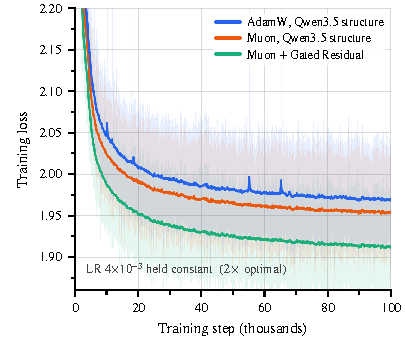
\includegraphics[pagebox=cropbox,width=\linewidth]{figs/paper_stress_2x_loss_half.pdf}
    \vskip -0.05in
    \caption{$2\times$ optimal learning rate.}
    \label{fig:stress-2x}
  \end{subfigure}
  \hfill
  \begin{subfigure}[t]{0.49\linewidth}
    \centering
    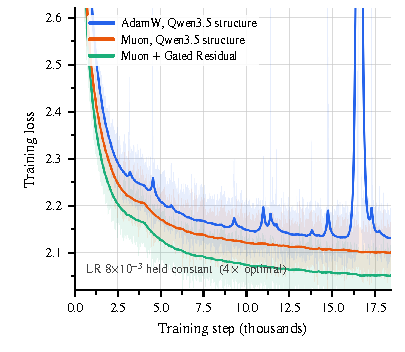
\includegraphics[pagebox=cropbox,width=\linewidth]{figs/paper_stress_4x_loss_half.pdf}
    \vskip -0.05in
    \caption{$4\times$ optimal learning rate.}
    \label{fig:stress-4x}
  \end{subfigure}
  \vskip -0.05in
  \caption{\textbf{Training loss under stress.} The 28-layer 25B-A3B MoE at a constant learning rate: the Qwen3.5 structure under AdamW, the same structure under Muon, and Muon with GR. Bold lines are a moving average over the faint per-step trace. GR enables more stable training.}
  \label{fig:stress-loss}
\end{figure}

\subsection{Stability Stress Test}
\label{sec:stability}


\paragraph{Motivation.}
\label{sec:stability-motivation}
When a model scales to trillions of parameters and is trained on tens of trillions of tokens, it enters a regime where stability challenges emerge that are entirely absent in smaller-scale experiments~\citep{chowdhery2023palm,zhang2022opt,dehghani2023vit22b,qwenteam2026qwen35}. 
For example, long training runs can spend substantially more optimizer steps at peak learning rates, increasing the opportunity for instabilities to emerge. 
Such instabilities often manifest as loss spikes or divergence that require checkpoint restarts.
To iterate efficiently at moderate scale while still surfacing the instabilities that would appear at production scale, we design a set of stress tests that amplify the relevant stress within a smaller budget.
This verification becomes essential when the architecture and optimizer change together, as they do in Qwen3.8-Flash-Next: the gated residual, the GDN hybrid, and Muon all alter how updates and activations are scaled, and confirming that these changes remain stable under prolonged training is a prerequisite for reliable scaling.


\paragraph{Stress Test Design.}
\label{sec:stability-method}
Following the observation that large-scale instabilities can be reproduced in small models by raising the learning rate~\citep{wortsman2023smallscale}, we hold the learning rate constant at a multiple of its optimal value, bypassing the standard decay schedule to simulate the prolonged peak learning rate of a production run. We apply this to a 28-layer MoE at $2\times$ and $4\times$ its optimal learning rate. The evaluation criterion is that the new recipe must be at least as stable as the previous Qwen3.5 structure with AdamW~\citep{qwenteam2026qwen35}, which has already been scaled successfully. 
All runs share the same batch size and a gradient-norm clipping threshold of $0.5$~\citep{pascanu2013clipping}. 
We measure three quantities: loss spikes (steps exceeding a $201$-step rolling median by more than $0.1$), the
$p_{99.9}$ of the pre-clip gradient norm and the number of threshold crossings, and the per-block maximum activation. 



\paragraph{Stress Test Results.}
\label{sec:stability-stress}
The stress tests reveal a clear stability margin for the new recipe. 
At $2\times$ the optimal learning rate, the AdamW baseline begins to spike ($4.3$ per $10$k steps), while both Muon configurations remain highly stable ($0.2$ per $10$k steps). 
At $4\times$ the optimal learning rate, the differences become categorical (Fig.~\ref{fig:stress-loss}). 
The AdamW run spikes on $183$ per $10$k steps and crosses the clipping threshold on $213$ of $19{,}932$ steps, engaging the clipper continuously. 
In contrast, both Muon runs never cross the clipping threshold, and the configuration with the gated residual records zero loss spikes. 
Under equal stress, the new architecture and optimizer combination is substantially more stable.

\begin{figure}[t]
  \centering
  \begin{subfigure}[t]{0.49\linewidth}
    \centering
    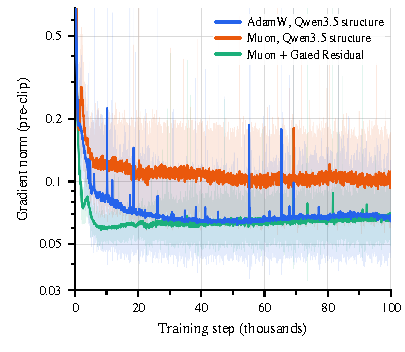
\includegraphics[pagebox=cropbox,width=\linewidth]{figs/paper_stress_2x_gnorm_half.pdf}
    \vskip -0.15in
    \caption{Pre-clip gradient norm.}
    \label{fig:stress-gnorm}
  \end{subfigure}
  \hfill
  \begin{subfigure}[t]{0.49\linewidth}
    \centering
    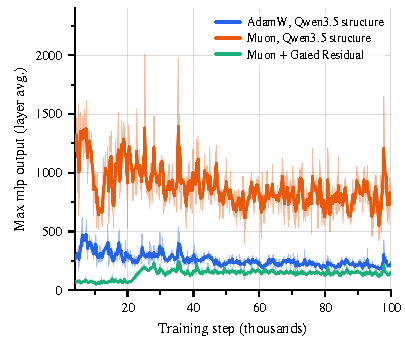
\includegraphics[pagebox=cropbox,width=\linewidth]{figs/paper_stress_2x_actmlp_half.pdf}
    \vskip -0.15in
    \caption{Maximum MLP output.}
    \label{fig:stress-actmlp}
  \end{subfigure}
  \vskip -0.05in
  \caption{\textbf{Gradient norm and activations under stress.} 
    The same three runs as Fig.~\ref{fig:stress-loss} (a). 
    The activation in (b) is averaged over layers. Gradient Residual reduces both the frequency and magnitude of gradient-norm spikes, as well as the magnitude of activation outliers (Fig.~\ref{fig:stress-mechanism}).}
  \label{fig:stress-mechanism}
\end{figure}


\begin{figure}[h]
  \centering
  \begin{subfigure}[t]{0.33\linewidth}
    \centering
    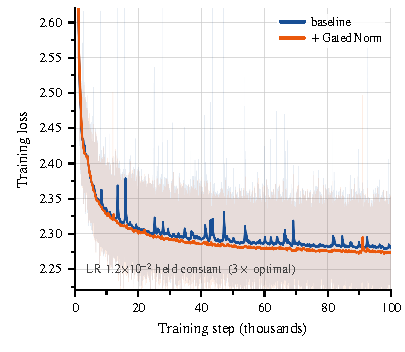
\includegraphics[pagebox=cropbox,width=\linewidth]{figs/paper_stress_gate_loss_half.pdf}
    \vskip -0.05in
    \caption{Training loss.}
    \label{fig:gate-loss}
  \end{subfigure}
  % \hfill
  \begin{subfigure}[t]{0.33\linewidth}
    \centering
    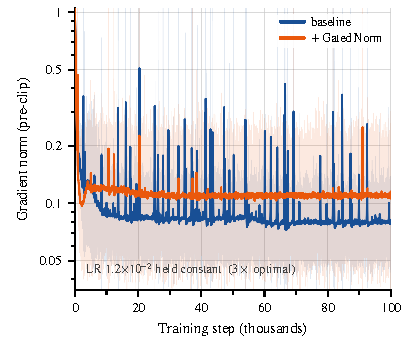
\includegraphics[pagebox=cropbox,width=\linewidth]{figs/paper_stress_gate_gnorm_half.pdf}
    \vskip -0.05in
    \caption{Pre-clip gradient norm.}
    \label{fig:gate-gnorm}
  \end{subfigure}
  % \vspace{4pt}
  \begin{subfigure}[t]{0.33\linewidth}
    \centering
    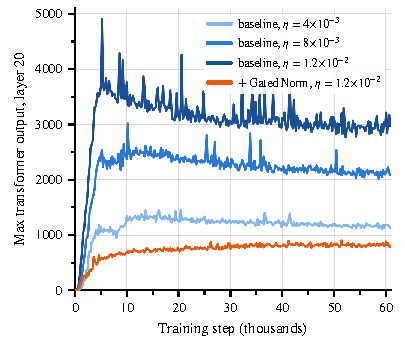
\includegraphics[pagebox=cropbox,width=\linewidth]{figs/paper_stress_gate_ladder_half.pdf}
    \vskip -0.05in
    \caption{Outliers against learning rate.}
    \label{fig:gate-ladder}
  \end{subfigure}
  \vskip -0.05in
  \caption{\textbf{Isolating the effect of the gate.} GatedNorm off and on, with the AdamW optimizer, structure and data order held fixed.
    \textbf{(a)} and \textbf{(b)} are the pair at $3\times$ the optimal learning rate; bold lines are a moving average over the faint per-step trace. \textbf{(c)} adds the ungated
    baseline at $1\times$ and $2\times$ the optimal rate.}
  \label{fig:gate}
\end{figure}

\paragraph{Mechanism: The Role of the Gate.}
\label{sec:stability-mechanism}
Analyzing the gradient norms and activations provides insight into this stability margin. 
At $2\times$ the optimal learning rate, Muon runs exhibit a higher median gradient norm and larger maximum activations than AdamW, yet they produce far fewer loss spikes. 
Adding GR reduces both the frequency and magnitude of gradient-norm spikes, as well as the magnitude of activation outliers (Fig.~\ref{fig:stress-mechanism}). 


To isolate the effect of the gate, we evaluate a single-variable pair on the 28-layer model at $3\times$ its optimal learning rate, keeping the AdmaW optimizer and structure fixed while toggling GatedNorm (Fig.~\ref{fig:gate}). 
Enabling the gate reduces the spike rate from $32.0$ to $3.2$ per $10$k steps and cuts threshold crossings from $256$ to $20$. 
A learning-rate ladder on the ungated baseline shows that activation outliers grow almost proportionally with the learning rate, while the spike rate grows much faster (Fig.~\ref{fig:gate-ladder} (c)). 
With the gate enabled at the highest learning rate, the outlier level drops below the baseline at the lowest learning rate. 
This suggests that training at high learning rates requires a rescaling mechanism: without an explicit gate, the network achieves this by growing activation outliers, leaving it fragile; the multiplicative gate supplies the necessary rescaling directly, keeping the training  stable~\citep{qiu2025gated,qiu2026unified}.





\begin{figure}[h]
  \centering
  \begin{subfigure}[t]{0.9\linewidth}
    \centering
    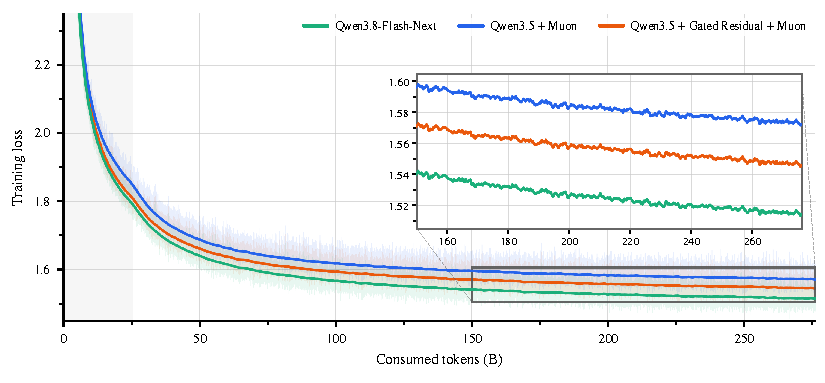
\includegraphics[pagebox=cropbox,width=\linewidth]{figs/paper_early_loss_wide.pdf}
    \vskip  -0.1in
    \caption{Training loss.}
    \label{fig:early-loss}
  \end{subfigure}
  \begin{subfigure}[t]{0.45\linewidth}
    \centering
    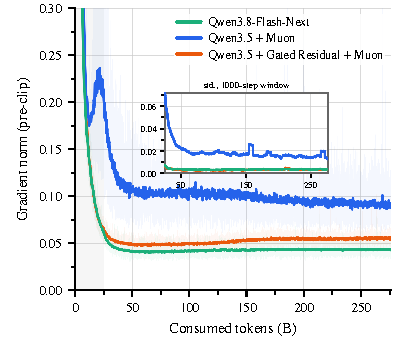
\includegraphics[pagebox=cropbox,width=\linewidth]{figs/paper_early_gnorm_half.pdf}
    \vskip  -0.1in
    \caption{Pre-clip gradient norm and sliding window std.}
    \label{fig:early-gnorm}
  \end{subfigure}
  \vspace{4pt}
  \begin{subfigure}[t]{0.45\linewidth}
    \centering
    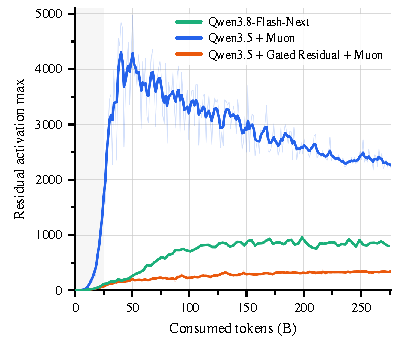
\includegraphics[pagebox=cropbox,width=\linewidth]{figs/paper_early_actmax_half.pdf}
    \vskip -0.05in
    \caption{Residual maximum over training.}
    \label{fig:early-actmax}
  \end{subfigure}
  \vskip -0.05in
  \caption{\textbf{The early phase of Qwen3.8-Flash-Next, at the shipped learning rate.} 
    % The first 276B tokens of three runs of one MoE that share data order, learning-rate schedule and optimizer: Qwen3.5 with Muon, the same plus the gated residual, and Qwen3.8-Flash-Next. 
    The first 276B tokens of three runs that share data order, learning-rate schedule, and optimizer: Qwen3.5 with Muon, the same plus the gated residual, and Qwen3.8-Flash-Next.
    The shaded band corresponds to the learning-rate warmup. The inset in (a) resolves the last $126$B tokens of the window; the inset in (b) is the standard deviation of the gradient norm
    inside a rolling $1000$-step window. 
    % The residual maximum in (c).
    }
  \label{fig:early}
\end{figure}

\paragraph{Verification at the Production Run.}
\label{sec:stability-production}
While the stress test amplifies instabilities by leaving the shipped
configuration, we also verify that the stability benefits persist under the
actual production training configuration. We compare the first $276$B tokens
of three runs sharing the same data order, learning-rate schedule, and
optimizer: the Qwen3.5 structure with Muon, the same structure plus GR, and
the full Qwen3.8-Flash-Next recipe with the further refined GR and the n-gram
embedding layer.

On loss (Fig.~\ref{fig:early}a), adding GR lowers the loss at $276$B tokens
by $0.026$, and the full Flash-Next recipe lowers it by a further
$0.032$, for a total gain of $0.058$ over the Muon baseline. This loss
improvement translates into significant benchmark gains
(\S\ref{sec:pt_eval}), enabling Qwen3.8-Flash-Next to reach pre-training
results comparable to Qwen3.7-Plus at roughly a ninth of the training
cost.

On gradient norm (Fig.~\ref{fig:early}b), Muon on its own has roughly twice the median norm and $4.2\times$ the $p_{99.9}$ of either gated run ($0.097$/$0.298$ vs.\ $0.053$/$0.071$ and $0.043$/$0.066$), and is the only
run to cross the clipping threshold. 
The gated runs are also steadier, with $4.3$--$4.7\times$ lower standard deviation inside a $1000$-step window, reproducing the stress-test finding at $8\times$ the model scale and at the production learning rate. 
Fusing the residual read and the final normalization before the LM head into one gated read operation further
reduces the gradient norm, likely the main contributor to the gap between Flash-Next and the Muon + GR configuration.
On activations (Fig.~\ref{fig:early}c), adding GR markedly reduces the
residual maximum throughout the network, consistent at every probed depth.
This allows stable training without explicit activation control such as qk-clip~\citep{kimi2025k2} and SwiGLU-clip~\citep{agarwal2025gpt}.